\chapter{Analisi dataset} \label{chap:Dataset}
In questa seconda parte l'obiettivo è quello di ricercare una correlazione tra gli errori scatenati durante la campagna di fault/error injection e le metriche estratte da Prometheus, in maniera tale da mostrare come sia possibile utilizzare tali metriche per creare apposite regole di alerting e far attivare tempestivamente eventuali operazioni di troubleshooting.


\section{Dataset}
\subsection{Campagna injection}
La campagna di fault/error injection è stata condotta utilizzando \textbf{Mutiny}, un framework appositamente sviluppato per Kubernetes che consente di manipolare i messaggi scambiati tra le varie componenti del sistema. L'applicazione monitorata è un web server Flask, il quale risponde alle richieste dei client eseguendo elaborazioni casuali. Le manipolazioni dei messaggi possono avvenire durante la comunicazione \textbf{tra l'Apiserver e l'Etcd}, con la possibilità di influire direttamente sullo stato attuale o desiderato del cluster, oppure \textbf{tra le componenti e l'Apiserver}, sebbene in quest'ultimo caso sia più probabile che i messaggi vengano identificati come corrotti e rigettati dall'Apiserver stesso.
\\
Durante la campagna sono state eseguite tre principali tipologie di iniezione:
\begin{itemize} 
    \item \textbf{Bit flip}: viene invertito un singolo bit all'interno del messaggio. 
    \item \textbf{Data-type set}: viene impostato un valore boundary o errato, a seconda del tipo di campo interessato.
    \item \textbf{Message drop}: simula la mancata ricezione di un aggiornamento di stato del cluster, dovuta a vari motivi come richieste fallite, bug, etc...
\end{itemize}
Per garantire un dataset completo, le metriche di Prometheus sono state raccolte utilizzando node exporter \cite{Node-exporter}, kube-state-metrics \cite{Kube-state-metrics} e metriche personalizzate dell'applicazione. Queste metriche sono state ricavate per ogni singola esecuzione della campagna. In particolare, sono state effettuate 300 run di controllo (\textit{gold runs}), dai cui risultati sono stati estratti i valori di riferimento per confrontare le time series generate durante le 8.782 run di iniezione.


\subsection{Struttura dataset}
 La combinazione di metriche ottenute durante la campagna permette di estrarre informazioni riguardanti lo stato dei nodi, degli oggetti Kubernetes e dell'applicazione, offrendo una vista completa sullo stato di salute del sistema.
\\
I dati sui cui sono state effettuate le analisi però sono solo un subset dell'intero dataset della campagna, con un numero limitato di tipologie di metriche e di classi di dati.

\subsection{Classificazione}
Per poter effettuare un'analisi in maniera più sistematica, i risultati delle run durante la campagna sono stati classificati a seconda del tipo di errore \textbf{visto dall'utente}:

\begin{itemize}
    \item Nessun Impatto Significante (\textbf{NSI}).
    \item Higher Response Time (\textbf{HRT}), solo ritardi temporali.
    \item Intermittent Availability (\textbf{IA}), risposte di errore a intermittenza.
    \item Service Unreachable (\textbf{SU}), servizio irraggiungibile.
\end{itemize}
a seconda del tipo di errore al \textbf{livello di orchestrazione}, di cui nel subset sono presenti:
\begin{itemize}
    \item \textbf{LeR}: il numero di repliche pronte, Pod creati o endpoint è stabile e inferiore alla baseline.
    \item \textbf{MoR}: il numero di repliche pronte, Pod creati o endpoint è superiore alla baseline.
    \item \textbf{Net}: il numero di repliche pronte e Pod è corretto, ma alcuni non sono raggiungibili o utilizzati nel bilanciamento del carico.
\end{itemize}
ed a seconda di sotto quale tipologia di \textbf{workload} di orchestrazione si è verificato l'errore:
\begin{itemize}
    \item \textbf{Deploy}: crea nuovi Deployment e Pod correlati.
    \item \textbf{Scale}: aumenta il numero di repliche dei Deployment esistenti. 
    \item \textbf{Failover} / \textbf{Availab}: forza i pod ad essere rigenerati tramite l'iniezione di un errore.
\end{itemize}

\begin{figure} [ht]
    \centering
    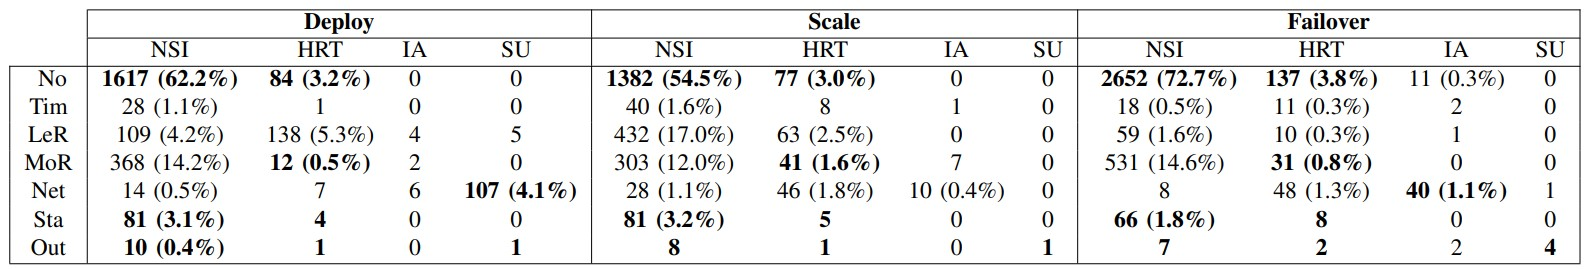
\includegraphics[width=1\linewidth]{UNINA_BSc_Final_Report//img//explanation/failure_full_map.jpg}
    \caption{risultati campagna di injection mappati errori - workload}
    \label{fig:of-cf-map}
\end{figure}

\section{Analisi}
L'approccio scelto per analizzare le metriche di Prometheus a disposizione è quello di realizzare dei grafi che permettano di visualizzare l'andamento delle metriche nei diversi scenari di errore a livello orchestrazione e per tipologia di workload. \\
Per fare ciò è stato realizzato un \textbf{notebook Jupyter} \cite{Jupyter}, che permette di caricare il dataset in memoria per poi scegliere singolarmente quali grafi realizzare in un secondo momento. Questo è possibile in quanto il flusso per generare un grafo è composto da 3 step separati: il caricamento del dataset in memoria, l'elaborazione dei dati per semplificarne l'utilizzo ed infine la generazione del grafo. \footnote{il notebook intero è reperibile sul repository GitHub \cite{github-repo}}

\subsection{Codice}
\subsubsection{Caricamento dati}

Nel dataset le metriche seguono circa questa struttura: \\  
/\textit{tipo errore orchestrazione}/\textit{[num. run]\_workload}/\textit{file metrica} \\
quindi per caricare i dati viene esplorato l'intero albero di directory, estrapolando i valori dai file delle metriche, file per file, per ottenere un array JSON [fig. \ref{fig:code-load-data}], dove una possibile riga è:
\begin{footnotesize}
\begin{verbatim}
{
    'metric': 
        {
            '__name__': 'node_memory_MemFree_bytes', 
            'instance': '192.168.100.20:9100'
        },
    'value': [1695843909.839, '1976422400'],
    'condition': 'Baselines', 'workload': 'deploy'
}
\end{verbatim}
\end{footnotesize}
in cui possiamo osservare il tipo di metrica, la time series (timestamp + valore), se la time series fa parte di una gold run o di una delle run di iniezione e sotto quale workload è stata rilevata.
\begin{figure} [ht]
    \centering
    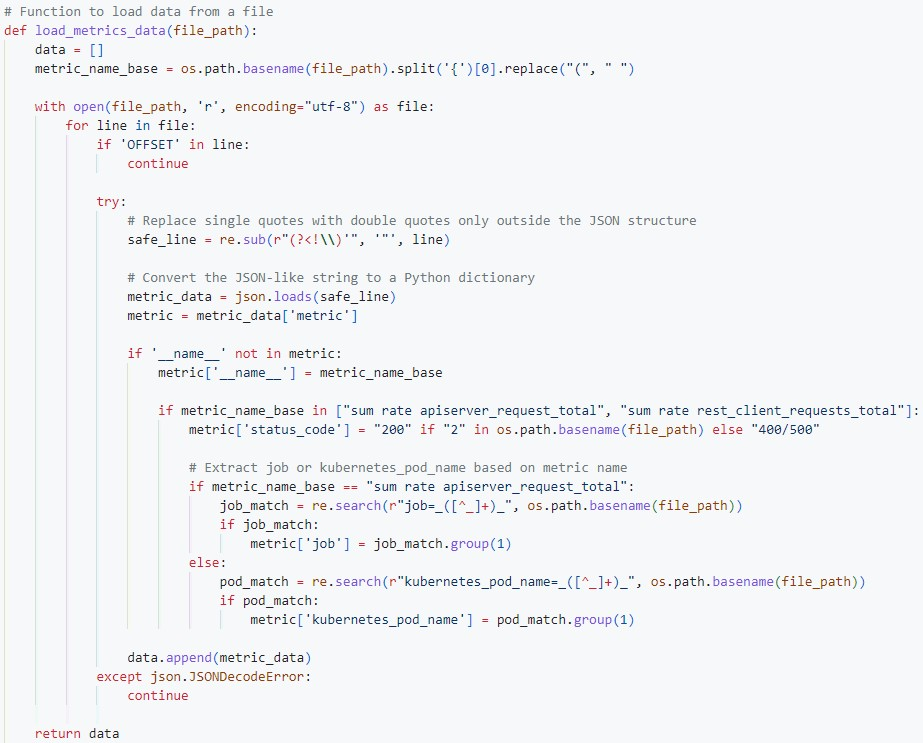
\includegraphics[width=0.8\linewidth]{UNINA_BSc_Final_Report//img//explanation/code_load_data.jpg}
    \caption{estrazione metrica in JSON}
    \label{fig:code-load-data}
\end{figure}

\subsubsection{Elaborazione dati}
Per poter lavorare più facilmente con i dati, l'array JSON viene convertito in un Dataframe della libreria Pandas \cite{code-pandas} [fig. \ref{fig:code-dataframe}], libreria che offre strutture dati e metodi per manipolare i dati.

\begin{figure} [ht]
    \centering
    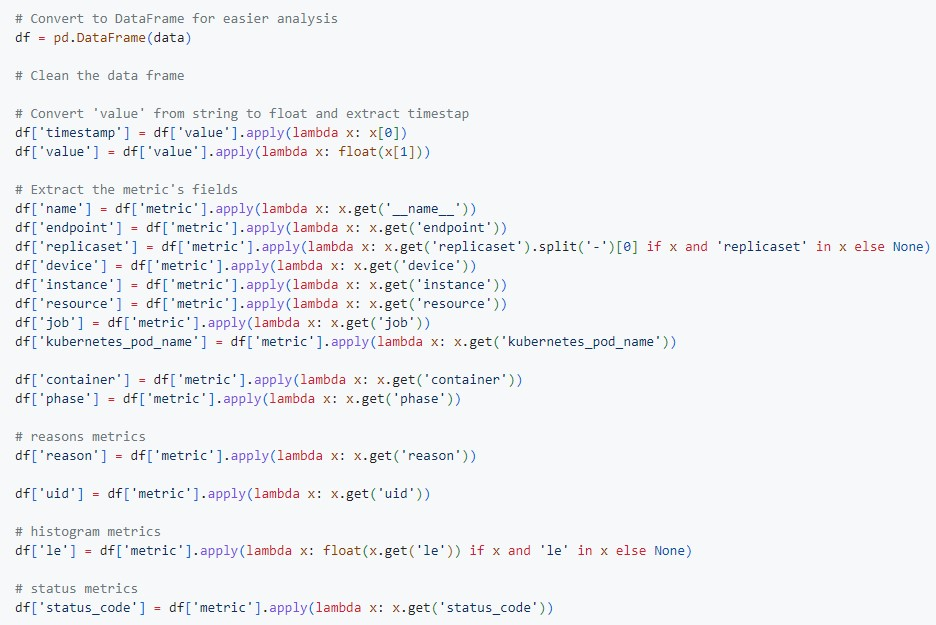
\includegraphics[width=0.9\linewidth]{UNINA_BSc_Final_Report//img//explanation/code_dataframe.jpg}
    \caption{conversione array JSON in Dataframe}
    \label{fig:code-dataframe}
\end{figure}

\subsubsection{Generazione grafi}
La generazione dei grafi avviene utilizzando la libreria \textbf{Matplotlib} \cite{code-matplotlib} e il suo toolkit \textbf{Seaborn} \cite{code-seaborn}, che semplifica la creazione dei grafi più comuni ed è compatibile con le funzionalità della libreria Pandas, grazie alle quali è stato possibile realizzare boxplot e heatmap [fig. \ref{fig:code-boxplot}].
\begin{figure} [!ht]
    \centering
    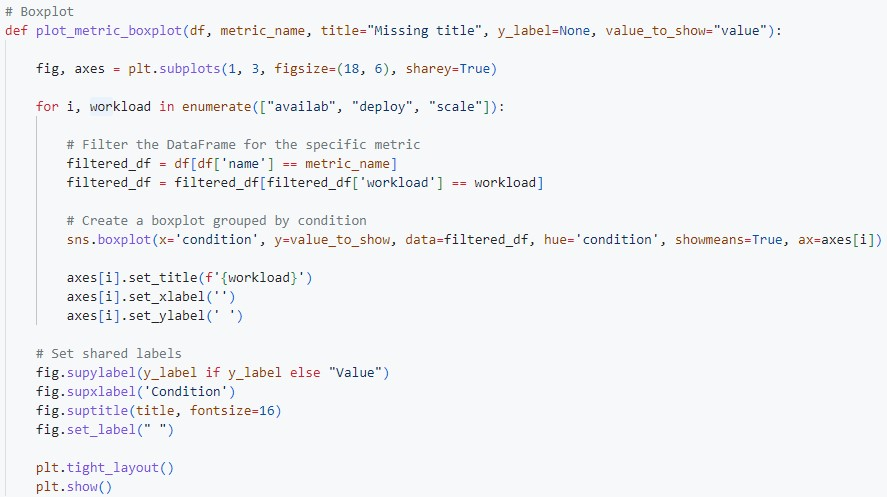
\includegraphics[width=0.9\linewidth]{UNINA_BSc_Final_Report//img//explanation/code_boxplot.jpg}
    \caption{codice boxplot}
    \label{fig:code-boxplot}
\end{figure}

\subsubsection{Boxplot e Heatmap} 
I box plot sono strumenti grafici utili per visualizzare la distribuzione di un insieme di dati. La scatola nel grafico rappresenta l'\textbf{intervallo interquartile} (\textbf{IQR}), con la linea centrale che indica la mediana, mentre i \textit{whisker} si estendono fino ai valori minimo e massimo, a meno che questi non siano considerati \textit{outlier} (valori anomali) [fig. \ref{fig:plot-boxplot-example}]. Questo tipo di grafico consente di identificare eventuali variazioni nell'andamento delle metriche in funzione della tipologia di errore e del carico di lavoro, permettendo un confronto chiaro delle diverse distribuzioni.

\begin{figure} [ht] \centering 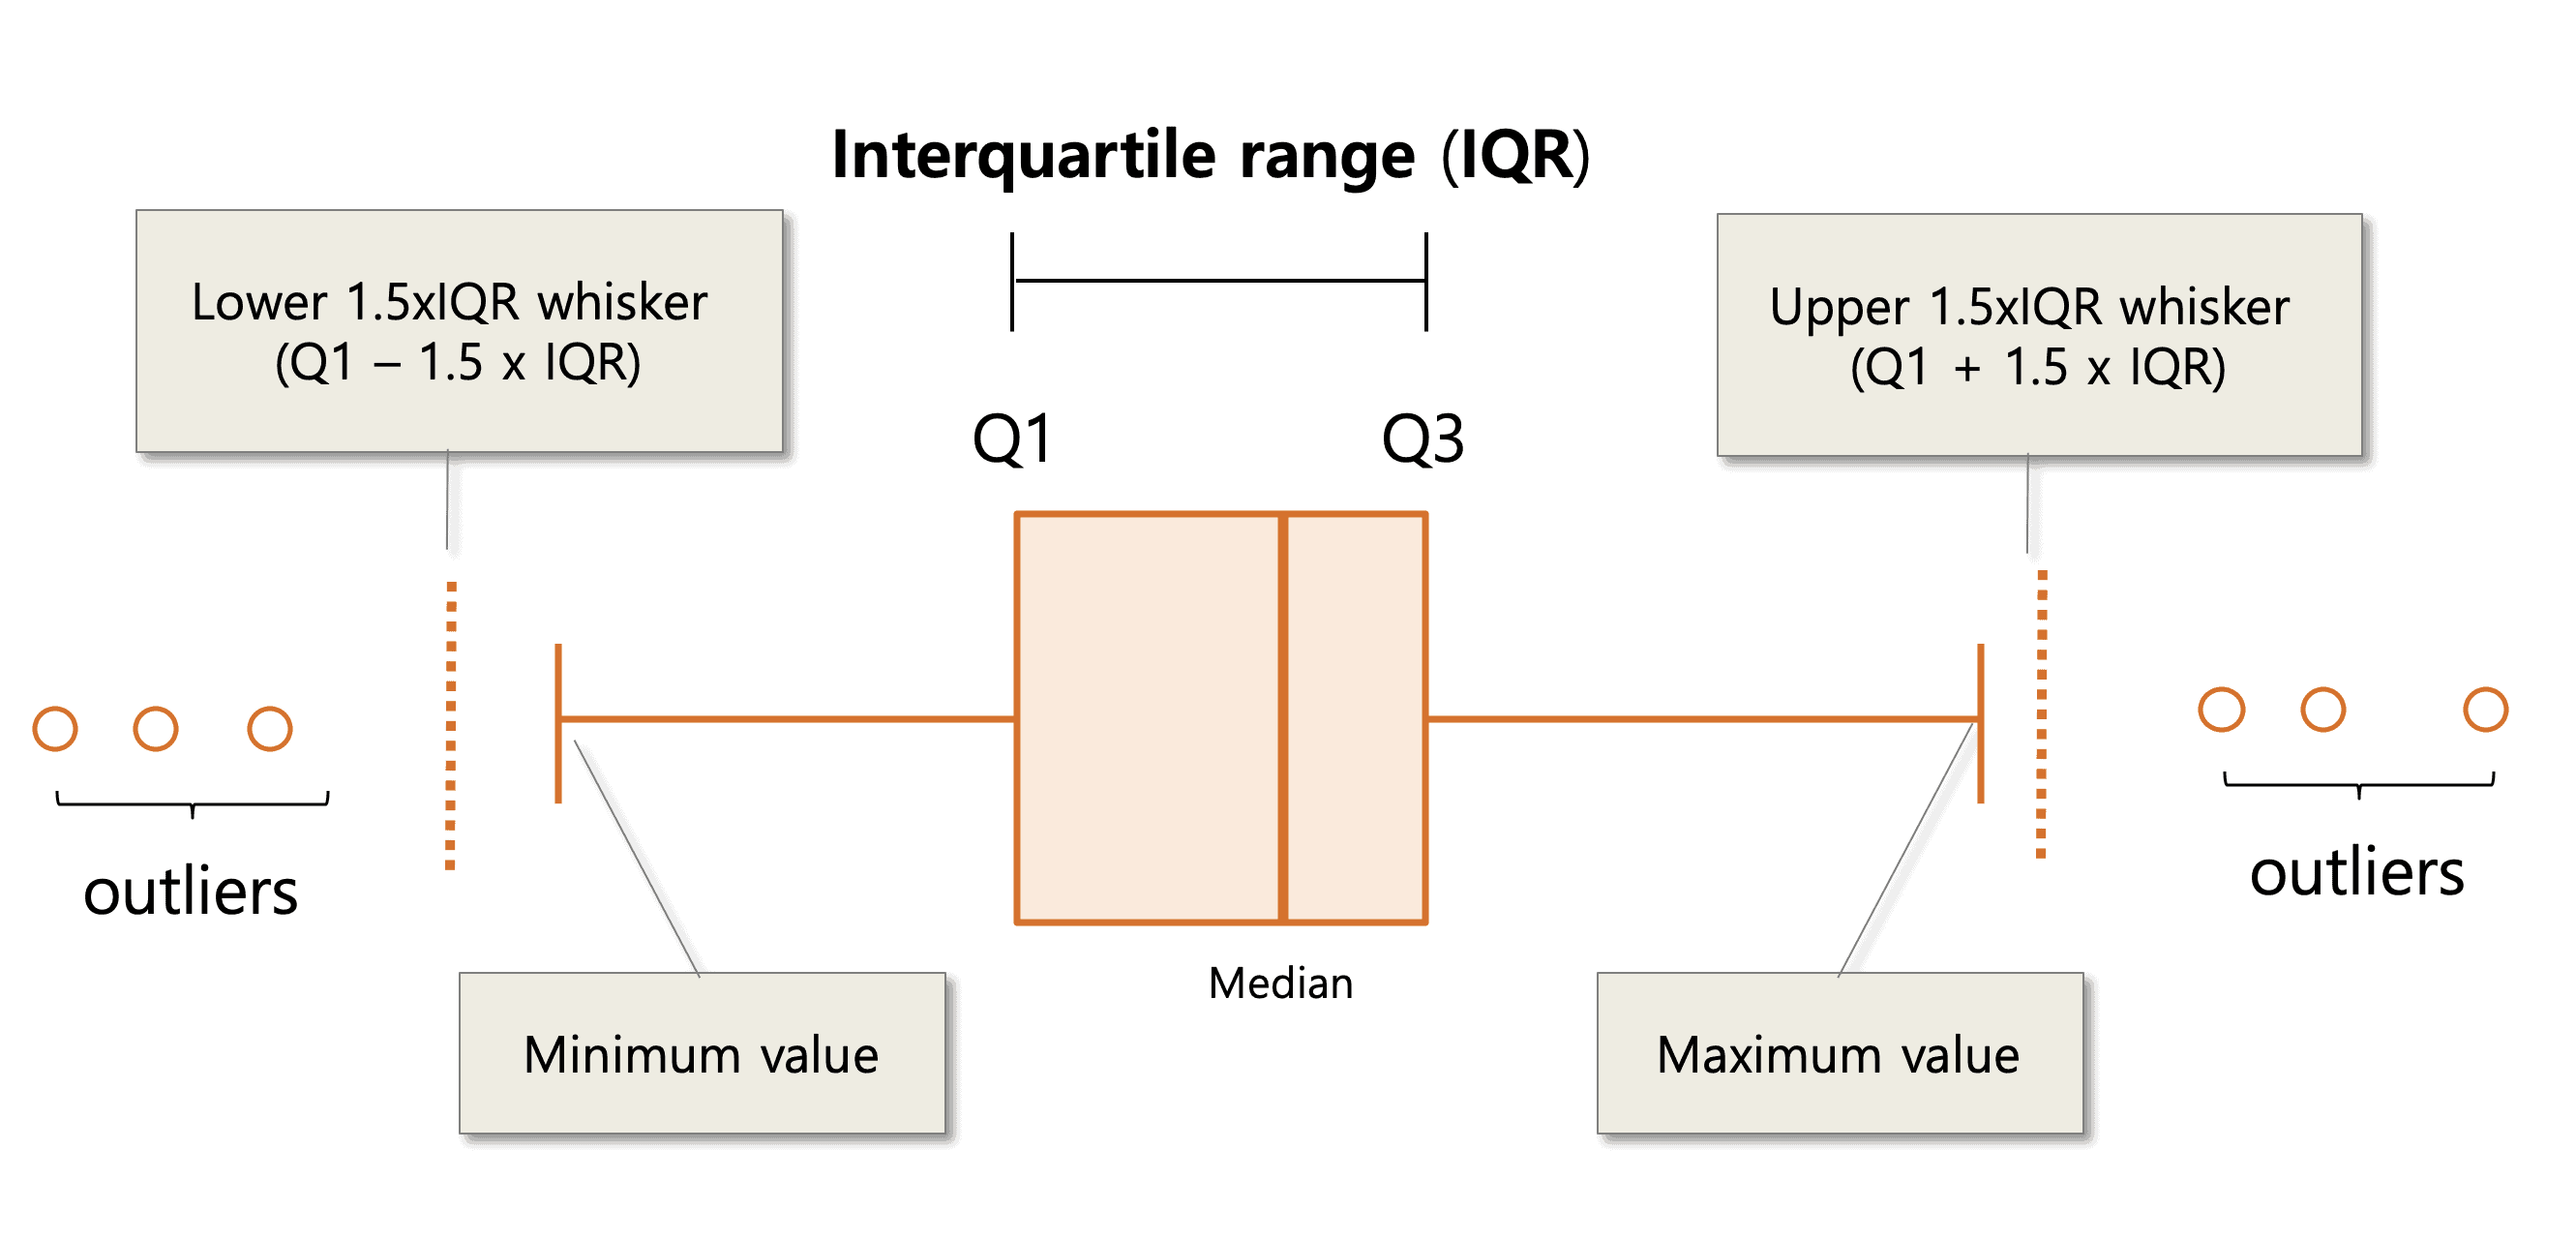
\includegraphics[width=1\linewidth]{UNINA_BSc_Final_Report//img//plots/boxplot-example.png} \caption{esempio di box plot \cite{boxplot-example}} \label{fig:plot-boxplot-example} 
\end{figure}

Le heatmap, invece, sono rappresentazioni grafiche che utilizzano una \textbf{scala di colori} per visualizzare la densità dei dati all'interno di un'area specifica. Nel contesto di questo lavoro, le aree rappresentano combinazioni tra il tipo di errore a livello di orchestratore e la tipologia di workload. Le zone con colori più intensi (zone "calde") indicano una maggiore concentrazione di dati, facilitando così l'individuazione di pattern o anomalie nelle distribuzioni [fig. \ref{fig:plot-heatmap-example}].

\begin{figure} [ht] \centering 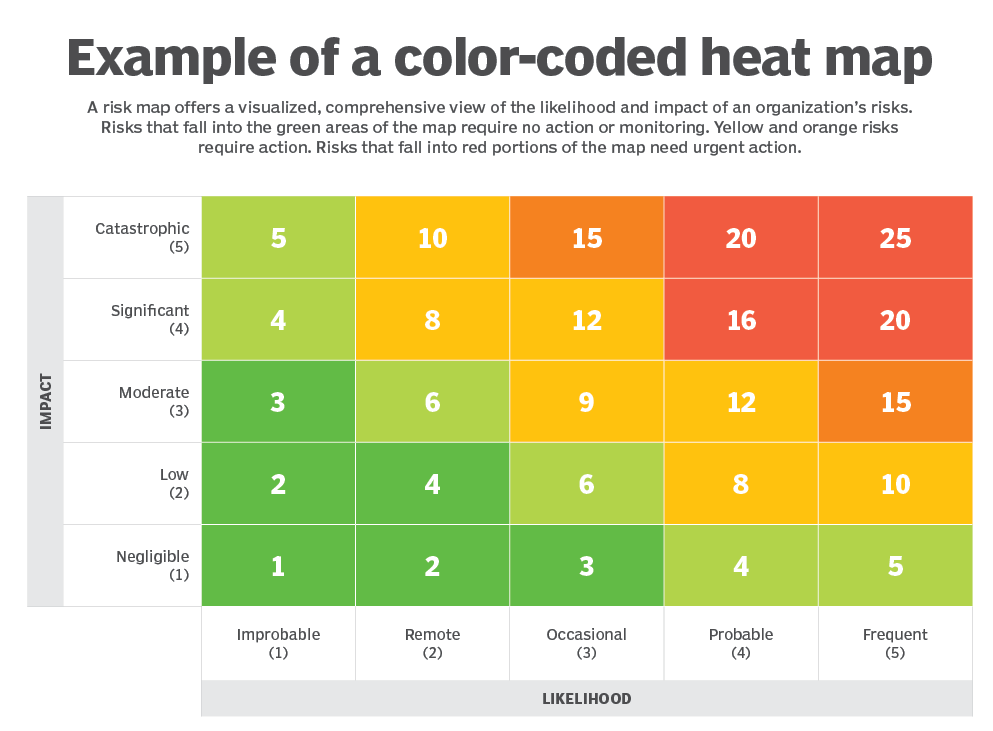
\includegraphics[width=0.8\linewidth]{UNINA_BSc_Final_Report//img//plots/heatmap-example.png} \caption{esempio di heatmap \cite{heatmap-example}} \label{fig:plot-heatmap-example}
\end{figure}

\subsection{Risultati}
Lavorando solo su un subset non è stato ovviamente possibile effettuare un'analisi completa, ma il processo utilizzato è facilmente estendibile a qualsiasi altra metrica.
Le metriche a disposizione sono circa 50, di cui diverse sono risultate essere non indicatrici di un \textbf{comportamento anomalo} come nel caso del ratio dei context switch al secondo dei processi nel nodo master [fig. \ref{fig:plot-useless-example}], dove non si osservano variazioni significative nell'intervallo interquartile (IQR), e le piccole variazioni presenti nei \textit{whisker} potrebbero essere influenzate da fattori esterni alla campagna di injection. \\
Di seguito verranno approfondite le metriche principali che hanno rilevato un comportamento anomalo per i possibili errori di orchestrazione confrontandole con il comportamento medio, che quindi possano effettivamente essere utilizzate per l'alerting o che quantomeno siano utili da monitorare.

\begin{figure} [ht]
    \centering
    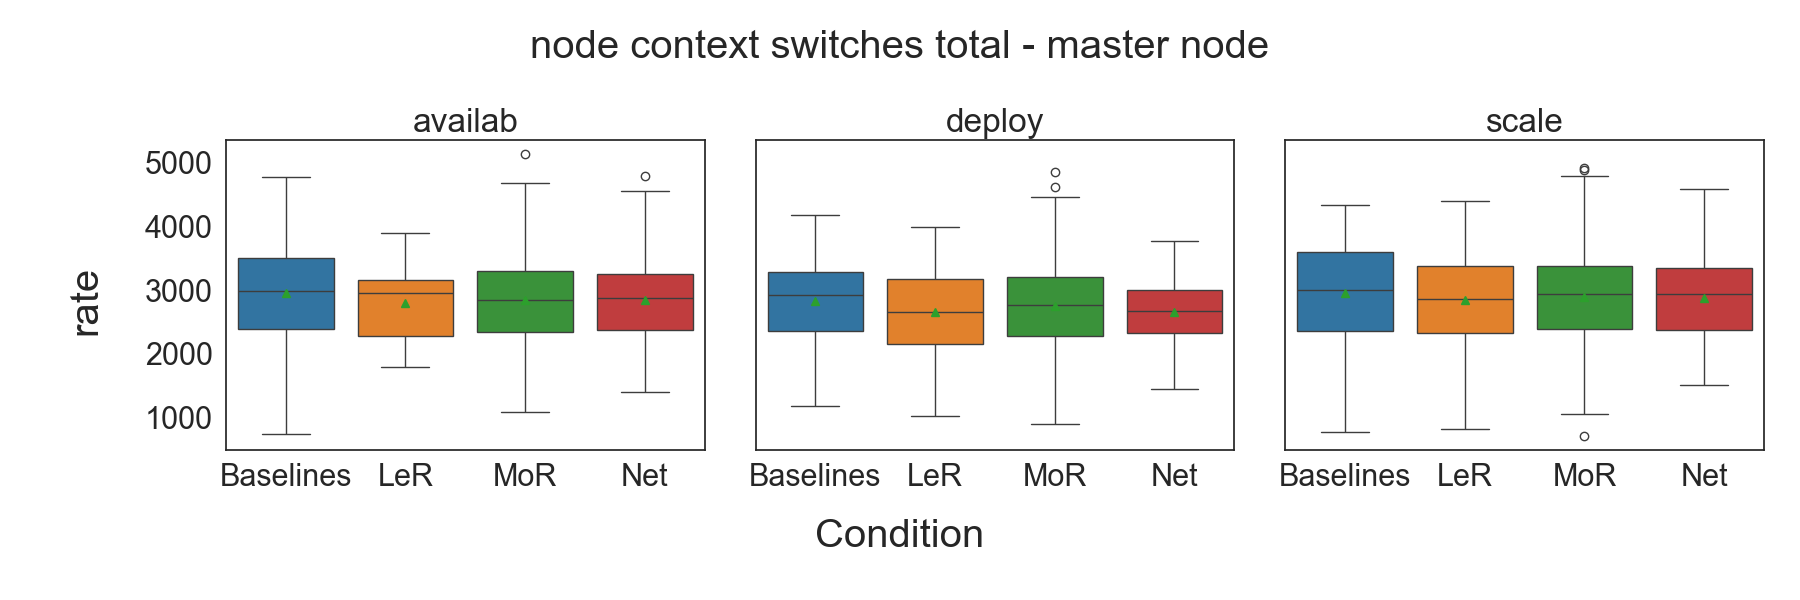
\includegraphics[width=1\linewidth]{UNINA_BSc_Final_Report//img//plots/node context switch - useless example.png}
    \caption{esempio di metrica non rilevante}
    \label{fig:plot-useless-example}
\end{figure}

\subsubsection{Utilizzo risorse}
\begin{figure}
    \centering
    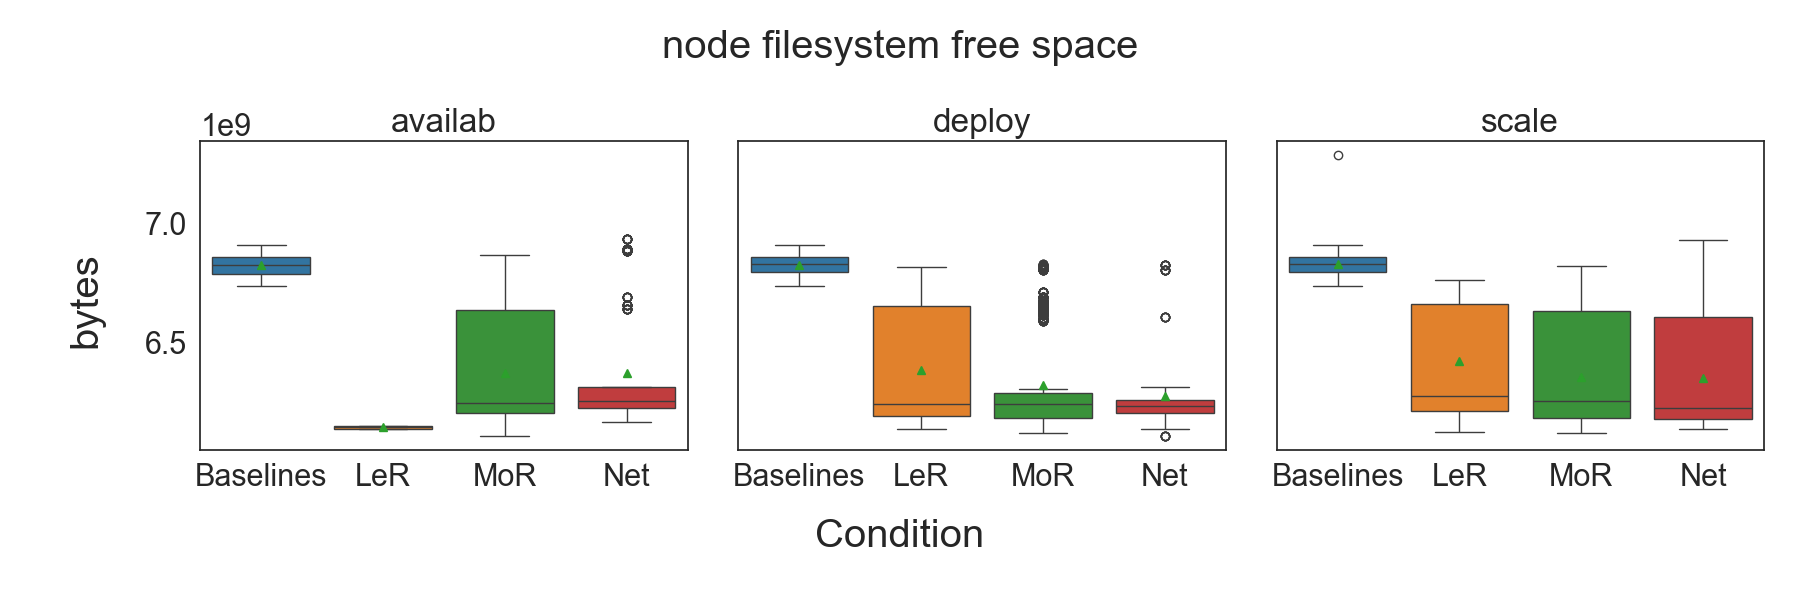
\includegraphics[width=1\linewidth]{UNINA_BSc_Final_Report//img//plots/node_free_fs_space.png}
    \caption{spazio libero del file system sul nodo in bytes \footnotesize(scala 10\(^9\))}
    \label{fig:plot-free-fs}
\end{figure}
Come si può osservare in tutte le condizioni di errore e sotto qualsiasi tipologia di workload, il nodo su cui è installato \textbf{il Control Plane utilizza decisamente più risorse} (circa 1 GB in più, sia sulla partizione del filesystem [fig. \ref{fig:plot-free-fs}] sia sulla memoria [fig. \ref{fig:plot-free-mem}], che su un nodo con 4 GB di ram è decisamente impattante), come si può evincere dal fatto che sotto tutti i workload, per entrambe le metriche, i whisker superiori degli errori non fanno nemmeno parte dell'IQR della baseline oltre ad avere una maggiore dispersione dei dati. Ad esempio il valore medio di memoria libero nel caso LeR sotto worload Availab è stato di circa 0.4 GB, mentre nel caso Baseline è di circa 1.7 GB. Questo probabilmente è il risultato di continue operazioni per cercare di portare lo stato del cluster allo stato desiderato senza mai riuscirci. 
\begin{figure} [!ht]
    \centering
    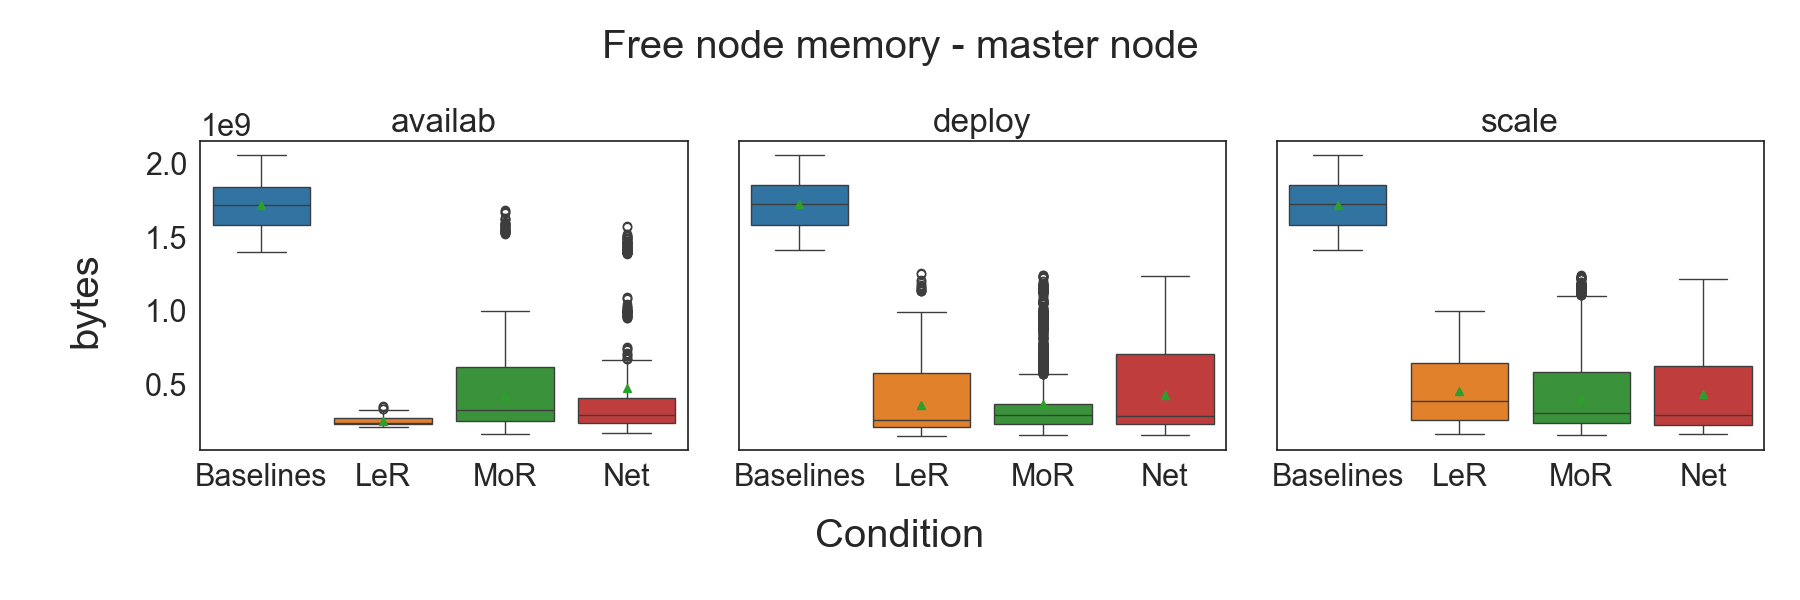
\includegraphics[width=1\linewidth]{node_free_mem.png}
    \caption{spazio libero in memoria sul nodo master in bytes \footnotesize(scala 10\(^9\))}
    \label{fig:plot-free-mem}
\end{figure} \\
In particolare nel caso di errori Net, la memoria disponibile subisce delle forti variazioni perché si verifica una condizione detta \textbf{capacity offset}, in cui la capacità dichiarata di un nodo è diversa dalla capacità effettivamente utilizzabile, a causa delle comunicazioni fallite tra Kubernetes ed il resto del sistema [fig. \ref{fig:plot-mem-net}]. Questa condizione non si verifica nei casi LeR e MoR perché viene proprio modificata la capacità delle risorse dei nodi dichiarata, anche se non corrisponde con l'effettiva capacità delle risorse fisiche del sistema.
\begin{figure}[!ht]
    \centering
    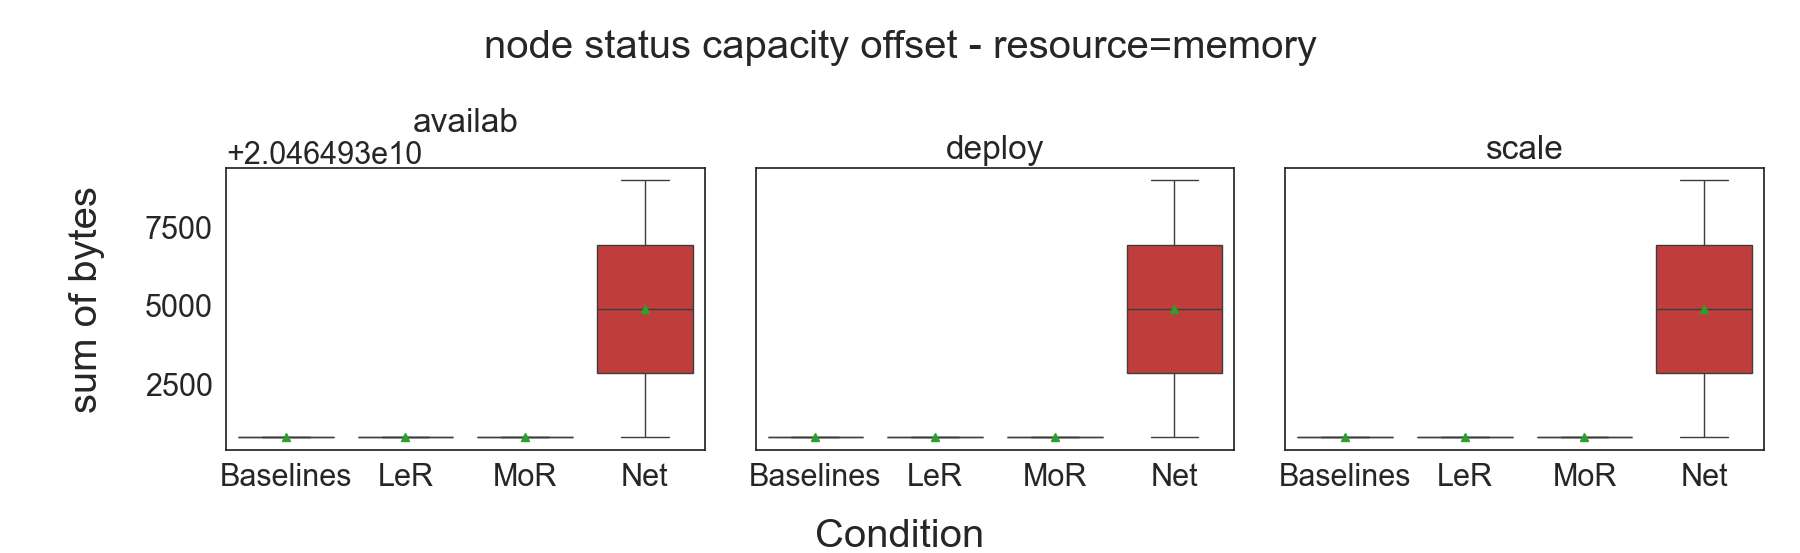
\includegraphics[width=1\linewidth]{UNINA_BSc_Final_Report//img//plots/sum kube_node_status_capacity_offset_offset_time)_by_ resource).png}
    \caption{discrepanza memoria utilizzabile e memoria dichiarata}
    \label{fig:plot-mem-net}
\end{figure}\\ \\ \\ 
Anche il ratio di utilizzo della CPU da parte dei processi può essere un ottimo indicatore, infatti nella condizione MoR si verificano diversi \textbf{picchi}, dove in alcuni casi quasi viene raggiunto il 100\% di utilizzo, indicati dai numerosi outliners, condizione che quindi si è verificata anche relativamente spesso e che può portare al crash dei pod e disservizi agli utenti [fig. \ref{fig:plot-cpu-ratio}].
\begin{figure} [ht]
    \centering
    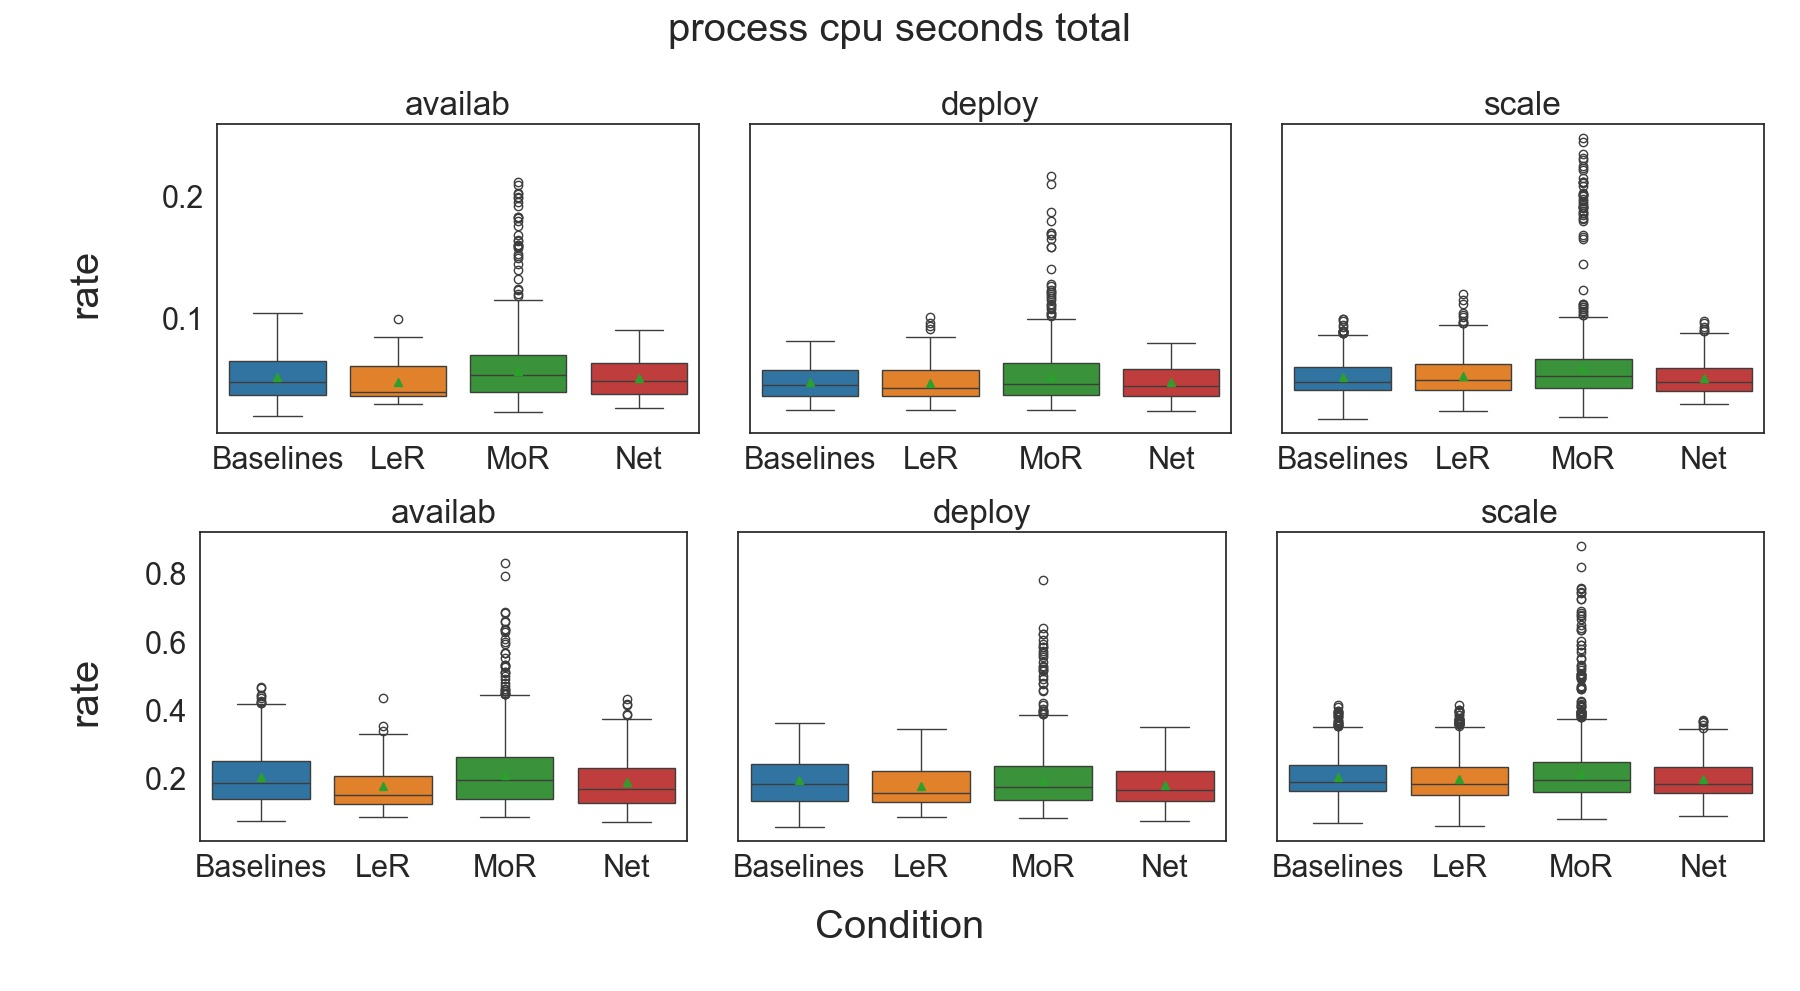
\includegraphics[width=0.8\linewidth]{UNINA_BSc_Final_Report//img//plots/rate process_cpu_seconds_total - all.jpg}
    \caption{ratio utilizzo cpu}
    \label{fig:plot-cpu-ratio}
\end{figure}

\subsubsection{Network}

Un'altra categoria di metriche da tenere sotto controllo riguarda le connessioni tra i nodi. Durante il workload di deploy, ovvero durante la creazione di nuovi pod o altri oggetti in Kubernetes, e in presenza di errori Net, sia il nodo master che i nodi worker tentano di stabilire un \textbf{numero elevato di nuove connessioni}. Questo comportamento si verifica perché molte delle connessioni falliscono, come evidenziato dall'ampiezza dell'intervallo interquartile (IQR) e dalla posizione elevata del whisker superiore. Tale fenomeno è visibile anche nella heatmap delle socket TCP in memoria, dove l'area deploy-Net è più scura rispetto alle altre.
In aggiunta, si osserva un significativo \textbf{incremento del numero di pacchetti inviati}, a cui segue un \textbf{aumento dei pacchetti ritrasmessi} a causa degli errori di comunicazione, chiaramente rilevabile nella heatmap del ratio dei pacchetti ritrasmessi, dove tale area è marcatamente più scura [fig. \ref{fig:plot-net-all}].
\begin{figure} [ht]
    \centering
    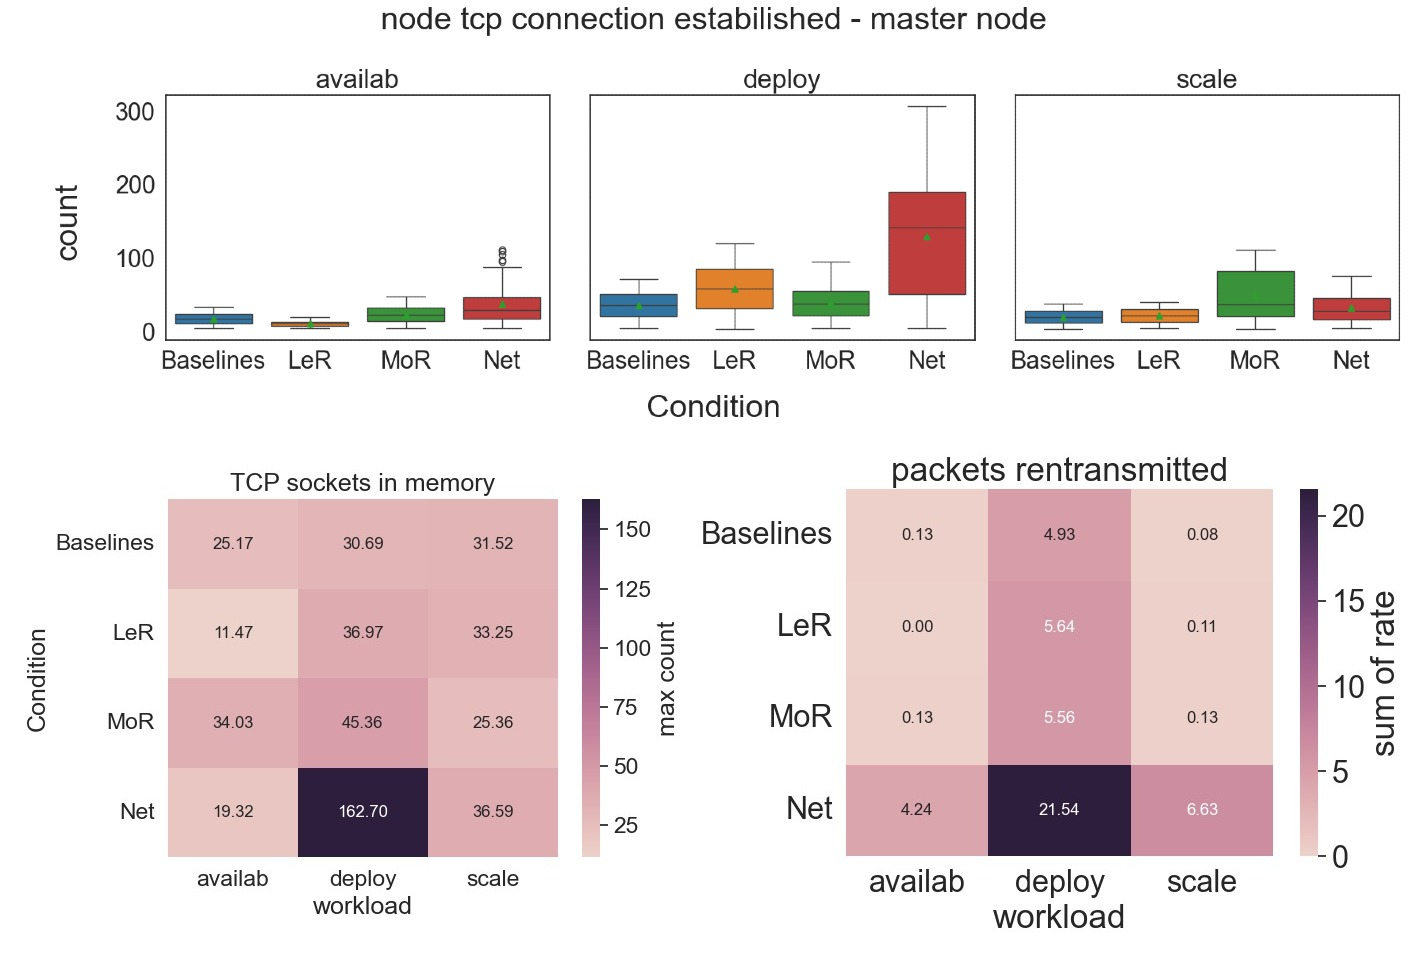
\includegraphics[width=1\linewidth]{UNINA_BSc_Final_Report//img//plots/Network - all.jpg}
    \caption{statistiche metriche di rete}
    \label{fig:plot-net-all}
\end{figure}


\subsubsection{Pod e container}

Lo stato dei pod e dei container va monitorato in maniera tempestiva, dato che sono un ottimo riferimento per controllare la salute dei servizi offerti.
In tutti i casi di errore si può osservare come i container dell'applicazione campione utilizzata nella campagna, \textbf{terminano numerose volte per errori} di diverso tipo, in particolar modo nel caso MoR, questo perché in generale tale problema risulta essere più critico rispetto agli altri dato che vengono assegnate più risorse di quelle disponibili [fig. \ref{fig:plot-pod-container}]. \\
Un altro dettaglio da notare è come nel caso di LeR sotto workload Failover, \textbf{i pod cambiano stato molto meno spesso mentre i container terminati per errore sono decisamente inferiori}, questo proprio perché avendo meno risorse a disposizione vengono creati meno pod e container, quindi una volta che sono stati terminati in maniera forzata molti non vengono più riavviati.
\begin{figure} [ht]
    \centering
    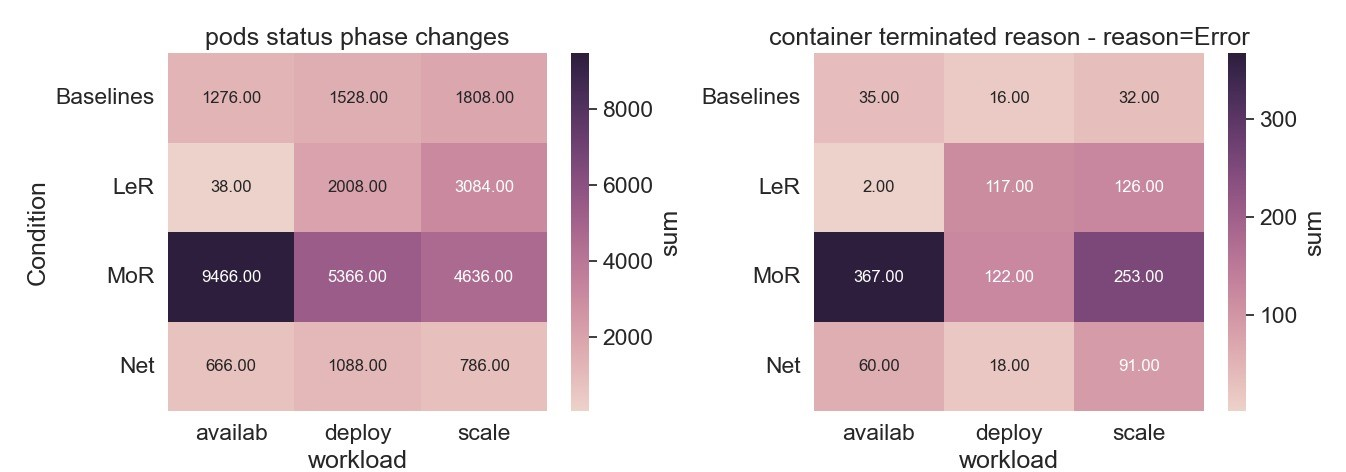
\includegraphics[width=1\linewidth]{UNINA_BSc_Final_Report//img//plots/pods - containers.jpg}
    \caption{variazioni stato pod e container terminati per errore}
    \label{fig:plot-pod-container}
\end{figure}

\subsubsection{Workqueue}

Lo stato delle workqueue permette anch'esso di identificare un eventuale sovraccarico del sistema, come avviene nel caso MoR in cui nelle queue vengono aggiunti spesso \textbf{più task rispetto alla media} [fig. \ref{fig:plot-queue-add}] credendo di avere maggiori risorse computazionali, situazione segnalata dai numerosi outliners, o addirittura nel caso di LeR sotto Failover risultano avere una \textbf{profondità quasi nulla} perché molti dei pod non vengono più riavviati risultando così in un carico molto più basso del normale [fig. \ref{fig:plot-queue-depth}].

\begin{figure} [ht]
    \centering
    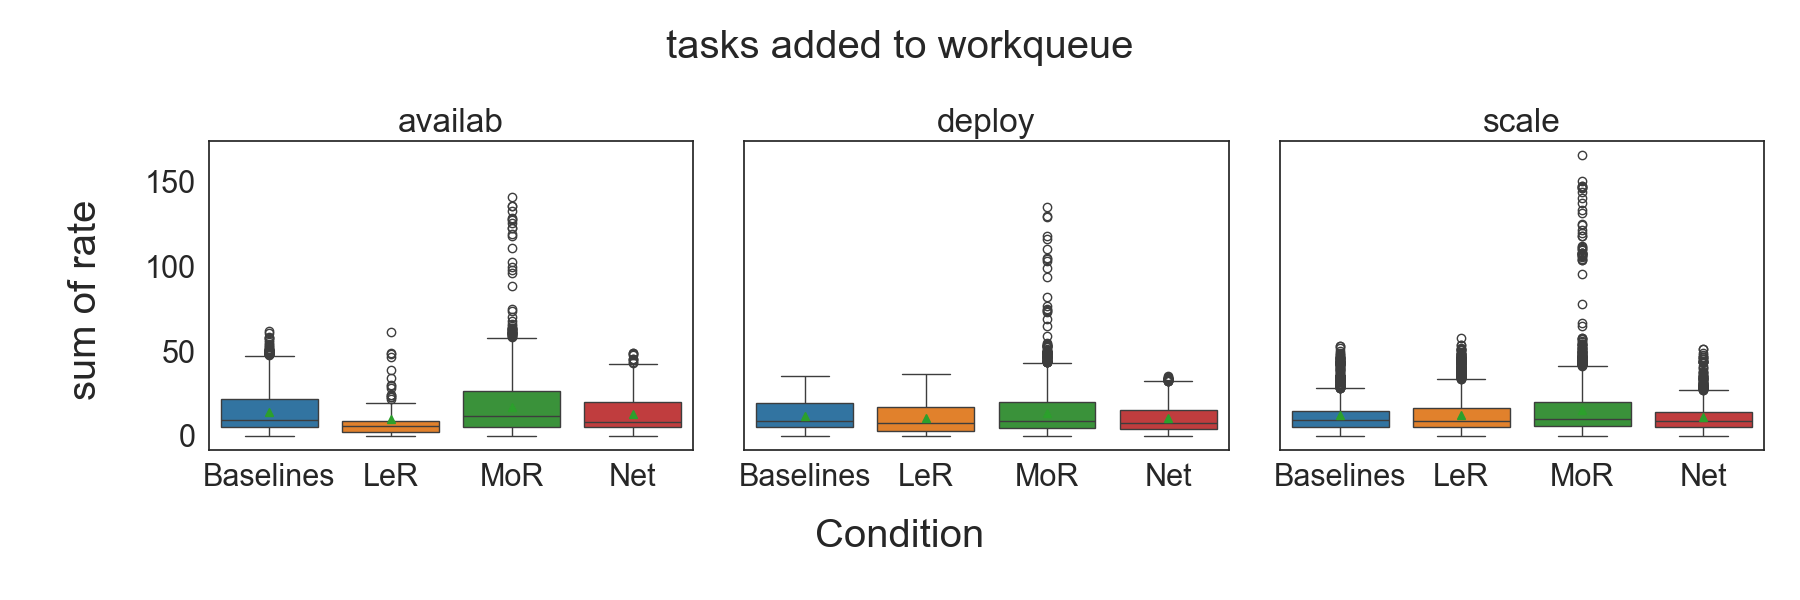
\includegraphics[width=0.9\linewidth]{UNINA_BSc_Final_Report//img//plots/workqueue_adds.png}
    \caption{inserimento task in una workqueue}
    \label{fig:plot-queue-add}
\end{figure}

\begin{figure}
    \centering
    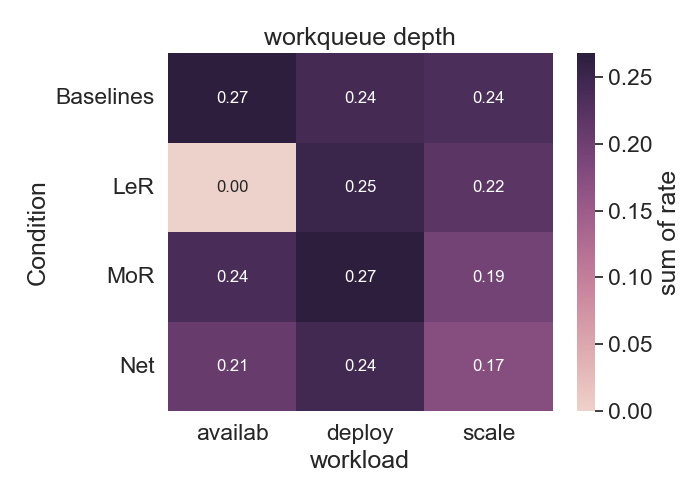
\includegraphics[width=0.5\linewidth]{UNINA_BSc_Final_Report//img//plots/workqueue_depth.png}
    \caption{profondità queue (LeR-Failover quasi nullo)}
    \label{fig:plot-queue-depth}
\end{figure}


\subsubsection{Metriche personalizzate}

Le metriche personalizzate create utilizzando le client library, permettono di monitorare in maniera più approfondita lo stato del servizio offerto, ad esempio con il server Flask utilizzato nella campagna possiamo controllare le \textbf{richieste HTTP ricevute} e relative \textbf{risposte} [fig. \ref{fig:plot-rest-request}]. Controllando ad esempio se in un determinato periodo di tempo le risposte di errore sono superiori alla media dato che nel caso MoR risultano essere particolarmente frequenti, situazione denotabile dai numerosi outliners, a causa del fatto che il BE accetta più richieste di quante possa effettivamente soddisfarne.
\begin{figure} [ht]
    \centering
    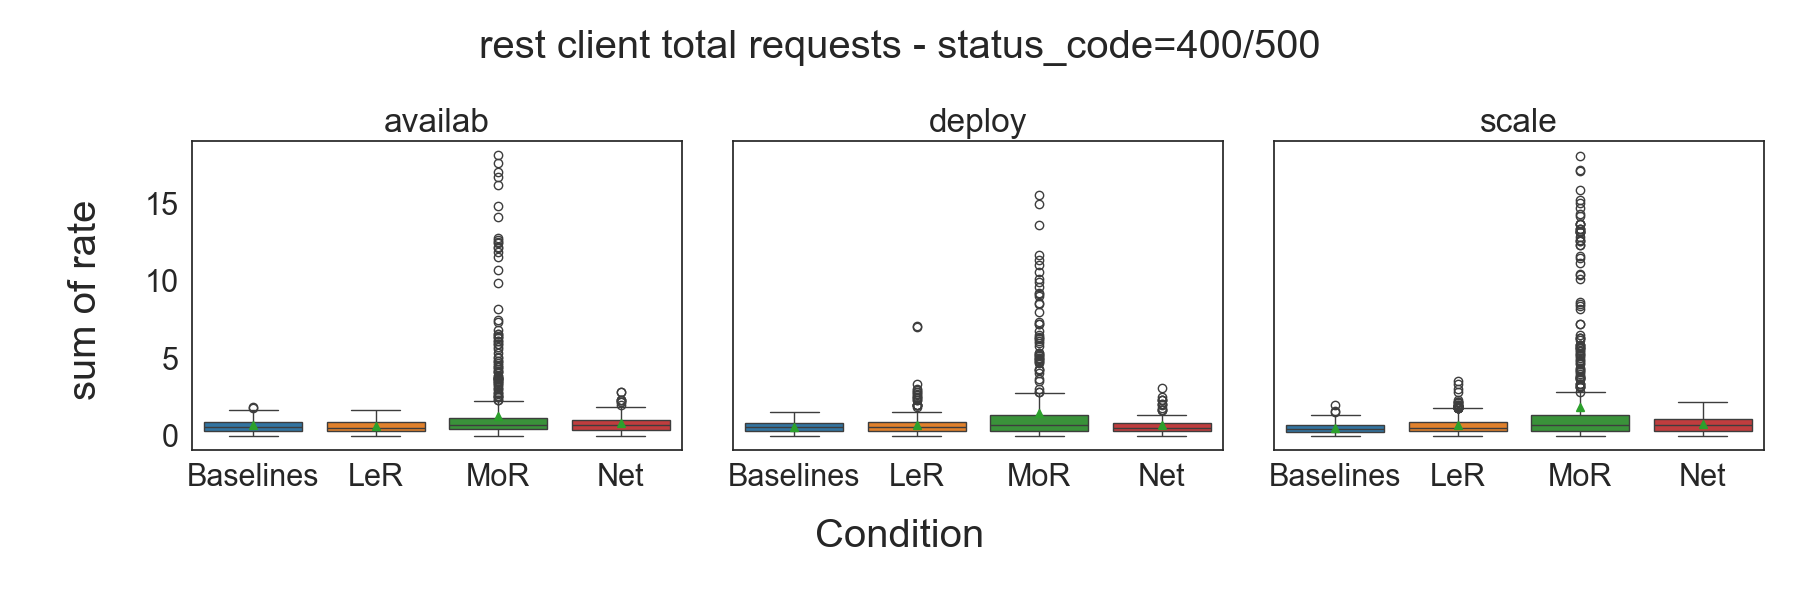
\includegraphics[width=0.9\linewidth]{UNINA_BSc_Final_Report//img//plots/rest requests.png}
    \caption{richieste HTTP con risposta 400/500}
    \label{fig:plot-rest-request}
\end{figure}


\subsection{Utilizzo delle metriche}

Per utilizzare efficacemente le metriche di Prometheus, è innanzitutto necessario ottenere un dataset iniziale che rappresenti lo stato di salute del cluster. Questo consente di stabilire un punto di riferimento per \textbf{identificare eventuali comportamenti anomali}, in maniera simile a quanto fatto precedentemente.\\
Tuttavia, per implementare delle regole di alerting basate su queste metriche, è essenziale definire soglie (\textbf{treshold}) di attivazione appropriate e considerare la possibilità di falsi positivi. Ad esempio, se consideriamo la metrica relativa allo spazio libero in memoria osservato nei nodi [fig. \ref{fig:plot-free-mem}], si può notare che in condizioni normali il nodo master dispone mediamente di circa 1.7 GB di memoria libera, mentre in caso di errore questo valore scende significativamente. Pertanto, si potrebbe impostare una soglia del 15\% inferiore alla media come limite di allerta, utlizzando una query PromQl come: \\
\textbf{\textit{node\_memory\_MemFree\_bytes < THRESHOLD}}
 \\
Con una soglia del 15\%, i falsi positivi risultano essere inferiori all'1\%, mentre il tasso di errori non rilevati è intorno al 2.7\%. Sebbene questi valori siano accettabili, è importante considerare che le variazioni nei dati non sono sempre così evidenti. Ad esempio, nel monitoraggio delle richieste HTTP con status code 400 o 500 [fig. \ref{fig:plot-rest-request}], tali eventi anomali possono essere isolati e limitati a brevi periodi di tempo. Per questo motivo, PromQL consente di \textbf{monitorare le metriche per un intervallo di tempo specifico}, permettendo di verificare, ad esempio, se negli ultimi 3 minuti si è verificato un numero di risposte negative significativamente superiore alla media.\\
\textbf{\textit{sum(rate(rest\_client\_requests\_total\{code=\textasciitilde"[45].."\} [3m] )) > THRESHOLD}}.

\subsection{Riepilogo metriche analizzate}
Le metriche che hanno rilevato un comportamento anomalo in uno o più casi di errore, presenti nel subset analizzato, sono state riepilogate nella tabella in fig. \ref{fig:plot-summary}, dove sono mappate le metriche, le tipologie di errore e i workload. Sono state segnate con un tick i casi in cui le metriche risultano essere utili da monitorare e sulla quale eventualmente applicarci regole di alerting. \\
\begin{figure} [ht]
    \centering
    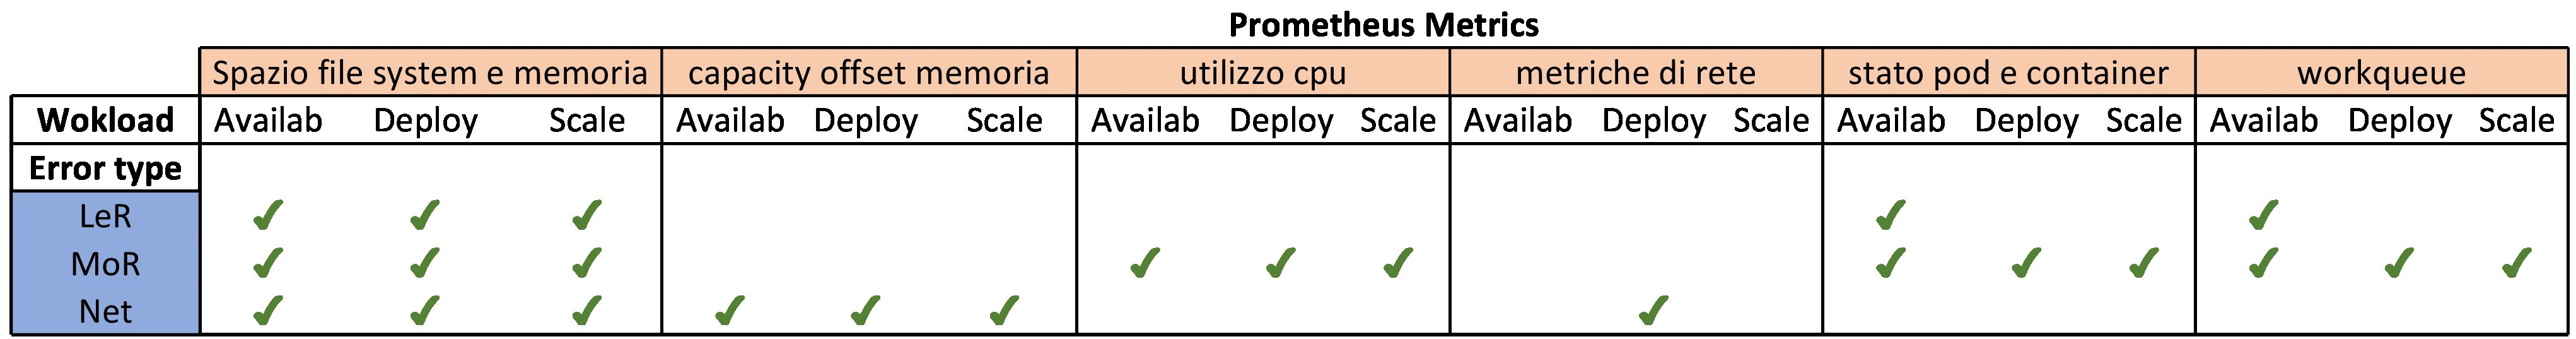
\includegraphics[width=1\linewidth]{UNINA_BSc_Final_Report//img//plots/map-metrics-error-workloads.jpg}
    \caption{mappa riepilogativa metriche - errori - workload}
    \label{fig:plot-summary}
\end{figure}

